Rewriting this in terms of $\rho$ we find:
\begin{align*}
	\sinh\frac{z}{b} &= \sqrt{\left(\frac{\rho}{b}\right)^2 - 1} \\
	\sinh^2\frac{z}{b} &= \left(\frac{\rho}{b}\right)^2 - 1 \\
	\frac{\rho}{b} &= \cosh \frac{z}{b}
\end{align*}
\begin{figure*}[h]
	\centering
	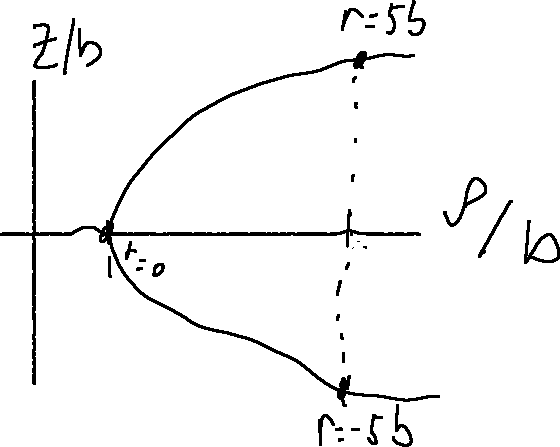
\includegraphics[width=6cm]{1-16-1.png}
	\caption*{Our embedding diagram}
\end{figure*}
Passing through $r=0$ here refers to moving to a distinct region of spacetime that is still flat but not the region of spacetime that we reached in the positive direction.
\subsection{Vectors in curved spacetime}
First we say that a vector is defined at a point in spacetime. Vector fields are generally functions of spacetime:
\begin{align*}
	\bm{a} &= \bm{a}(x^\mu)
\end{align*}
We now extend our basis vectors to be vector fields that are position dependant, i.e.:
\begin{align*}
	\bm{a} &= a^\alpha(x^\mu) \bm{e}_\alpha(x^\mu)
\end{align*}
So our dot product becomes:
\begin{align*}
	\bm{a}\cdot\bm{b} &= (\bm{e}_\alpha\cdot\bm{e}_\beta)a^\alpha b^\beta
\end{align*}
If we define a locally flat frame we conventionallly write: $\bm{e}_{\hat{\alpha}} \cdot\bm{e}_{\hat{\beta}} = \eta_{\hat{\alpha}\hat{\beta}}$.
These locally flat frames describe how an observer would view things. We do that by saying $\bm{e}_{\hat{t}} = \bm{u}_\text{obs}$.

Additionally we will have a coordinate basis where:
\begin{align*}
	u^\alpha &= \frac{dx^\alpha}{d\tau}
\end{align*}
Which in general will not be the same as our locally flat or orthonormal basis. We know that:
\begin{align*}
	\bm{u}\cdot\bm{u} &= -1 \\
	ds^2 &= g_{\alpha\beta}dx^\alpha dx^\beta \\
	ds^2 &= -d\tau^2
\end{align*}
We say we can write:
\begin{align*}
	g_{\alpha\beta}u^\alpha u^\beta &= -1
\end{align*}
In the coordinate basis.

To define the coordinate basis we say it is the basis in which:
\begin{align*}
	\bm{e}_\alpha(x^\mu)\cdot\bm{e}_\beta(x^\mu) &= g_{\alpha\beta}(x^\mu)
\end{align*}

So in summary we use our coordinate basis to do calculations, while we use orthonormal/locally flat basis to do interpretations. We will also use $\hat{\alpha}$ to refer to our orthonormal basis.

We now consider a coordinate basis and an orthonormal basis:
\begin{align*}
	\bm{a} &= a^\alpha\bm{e}_\alpha \\
	\bm{a} &= a^{\hat{\alpha}}\bm{e}_{\hat{\alpha}}
\end{align*}
In order to transform between these we need to express the components in terms of the other set of basis vectors, i.e:
\begin{align*}
	a^\alpha &= a^{\hat{\beta}}(\bm{e}_{\hat{\beta}})^\alpha \\
	a^{\hat{\alpha}} &= a^{\beta}(\bm{e}_{\beta})^{\hat{\alpha}}
\end{align*}
\subsection{Geodesics}
THe worldline of a free test particle between two timelike seperated points will exteremize the proper time between them. These extermized paths are known as geodesics, and the equations of motion that determine them are known as the geodesic equations.

For example we consider the equations for geodesics in plane in polar coordinates.
\begin{align*}
	dS^2 &= dr^2 + r^2 d\phi^2
\end{align*}
We describe a curve betwweeen two points $A$ and $B$ parametrically as $r(\sigma)$ and $\phi(\sigma)$, where $\sigma\in[0,1]$:
\begin{align*}
	S_{AB} &= \int_A^B dS \\
	S_{AB} &= \int_0^1 d\sigma \sqrt{\left(\frac{dr}{d\sigma}\right)^2 + r^2 \left(\frac{d\phi}{d\sigma}\right)^2}
\end{align*}
We can see that this defines a lagrangian:
\begin{align*}
	\mathcal{L}&= \sqrt{\left(\frac{dr}{d\sigma}\right)^2 + r^2 \left(\frac{d\phi}{d\sigma}\right)^2} \\
	\frac{d}{d\sigma} \left(\frac{1}{\mathcal{L}} \frac{dr}{d\sigma}\right) &= \frac{r}{\mathcal{L}} \left(\frac{d\phi}{d\sigma}\right)^2 \\
	\frac{d^2r}{ds^2} &= r\left(\frac{d\phi}{ds}\right)^2
\end{align*}

The equations for time-lke geodesics will be talked about in terms of proper time:
\begin{align*}
	\tau_{AB} &= \int_A^Bd\tau \\
	\tau_{AB} &= \int_A^B\sqrt{-g_{\alpha\beta}(x) dx^\alpha dx^\beta} \\
	\tau_{AB} &= \int_0^1d\sigma\sqrt{-g_{\alpha\beta}(x) \frac{dx^\alpha}{d\sigma} \frac{dx^\beta}{d\sigma}}
\end{align*}
Which gives us a Lagrangian:
\begin{align*}
	\mathcal{L} &= \sqrt{-g_{\alpha\beta}(x)\frac{dx^\alpha}{d\sigma}\frac{dx^\beta}{d\sigma}}
\end{align*}
Where:
\begin{align*}
	\partder{\mathcal{L}}{dx^\alpha} &= \frac{d}{d\sigma} \partder{\mathcal{L}}{\frac{dx^\alpha}{d\sigma}}
\end{align*}

We now return to our wormhole geometry:
\begin{align*}
	ds^2 &= -dt^2 + dr^2 + (r^2 + b^2)(d\theta^2 + \sin^2\theta d\phi^2) \\
	\mathcal{L} &= \sqrt{\left(\frac{dt}{d\sigma}\right)^2 - \left(\frac{dr}{d\sigma}\right)^2 0 (b^2 + r^2)\left[\left(\frac{d\theta}{d\sigma}\right)^2 + \sin^2\theta \left(\frac{d\phi}{d\sigma}\right)^2\right]}
\end{align*}
We note that $\partder{\mathcal{L}}{()} \propto \frac{1}{\mathcal{L}}$ and we also see:
\begin{align*}
	\mathcal{L} &= \frac{d\tau}{d\sigma} \\
	\partder{\mathcal{L}}{t} &= 9 &
	\frac{d^2 t}{d\tau^2} &= 0 \\
	\partder{\mathcal{L}}{r} &= -\mathcal{L}r\left[\left(\frac{d\theta}{d\sigma}\right)^2 + \sin^2\theta \left(\frac{d\phi}{d\sigma}\right)^2\right] \\
	\partder{\mathcal{L}}{\frac{dr}{d\sigma}} &= -\frac{d r}{d\tau}
\end{align*}
WHich then implies:
\begin{align*}
	\frac{d^2 r}{d\tau^2} &= r\left[\left(\frac{d\theta}{d\sigma}\right)^2 + \sin^2\theta \left(\frac{d\phi}{d\sigma}\right)^2\right] \\
\end{align*}
We now look at the rest of the problem:
\begin{align*}
	\frac{d}{d\tau} \left[(b^2 + r^2)\frac{d\theta}{d\tau}\right] &= (b^2 + r^2)\sin\theta\cos\theta\left(\frac{d\theta}{d\tau}\right)^2 \\
	\frac{d}{d\tau} \left[(b^2+ r^2)\sin^2\theta \frac{d\phi}{d\tau}\right] &= 0
\end{align*}

The general form of the geodesic equation for timelike geodesics will be:
\begin{align*}
	\frac{d^2x^\alpha}{d\tau^2} &= -\Gamma_{\beta\gamma}^\alpha \frac{dx^\beta}{d\tau} \frac{dx^\gamma}{d\tau}
\end{align*}
This is a set of for equations, one for each $\alpha$. The $\Gamma$ symbols are called the Christoffel symbols, are constructed from our metric and 1st derivitives, and are notably not tensors:
\begin{align*}
	u^z\alpha &= \frac{dx^\alpha}{d\tau} \\
	\frac{du^\alpha}{d\tau} &= -\Gamma_{\beta\gamma}^\alpha u^\beta u^\gamma
\end{align*}
These are symmetric in the lower indicies.
`
Looking back at the plane in polar coordinates:
\begin{align*}
	\frac{d^2 r}{dS^2} &= r \left(\frac{d\phi}{dS}\right)^2 &
	\frac{d}{dS} \left(r^2 \frac{d\phi}{dS} \right) &= 0 \\
	\Gamma_{\phi\phi}^r &= -r &
	\Gamma_{r\phi}^\phi &= \frac{1}{r}
\end{align*}
Where all the others will be 0.

We can additionally compute the Chrisoffel symbols via:
\begin{align*}
	g_{\alpha\delta}\Gamma_{\beta\gamma}^\delta &= \frac{1}{2}\left(\partder{g_{\alpha\beta}}{x^\gamma} + \partder{g_{\alpha\gamma}}{x^\beta} - \partder{g_{\beta\gamma}}{x^\alpha}\right)
\end{align*}
